\chapter{Scaling Latency}

\section{Bitcoin Latency}
In Bitcoin, when a transaction has been included in a block, it will be confirmed only after the block is buried $k$-deep in the longest chain. Furthermore, to ensure confirmation with high probability, $k$ must be large. The average latency of confirmation is then the product of $k$ and the average inter-block arrival time; again just like the throughput, the latency in Bitcoin is also limited by security. How bad is this trade off? In summary, we have:
\begin{itemize}
    \item \textbf{Confirmation in Bitcoin:} In Bitcoin, a transaction is confirmed when it is included in a block, which is then buried $k$-deep in the longest chain.
    \item \textbf{Latency of Confirmation:}  The average latency of confirmation is the product of $k$ and the average inter-block arrival time.
    \item \textbf{Trade-off with Security:} To ensure high probability of confirmation, $k$ must be large. However, this trade-off is limited by security concerns.
    \item \textbf{Analysis with Zero Network Delay:} The analysis begins with the assumption of zero network delay ($\delta = 0$).
    \item \textbf{Error Probability ($\epsilon$): }  The largest probability of deconfirmation is achieved by the private attack. The error probability ($\epsilon$) decays exponentially with the depth of the confirmation rule ($k$).
    \item  \textbf{Exponential Decay of Error Probability:} The error probability ($\epsilon$) is given by $\epsilon = e^{-ck}$, where $c = - log_{e}(4\beta(1 - \beta))$.
    \item \textbf{Parameters:} Here, $\beta$ represents the fraction of the hash power of the adversary.
\end{itemize}
This analysis demonstrates that the error probability decreases exponentially with an increase in the confirmation depth ($k$) and is influenced by the fraction of hash power controlled by the adversary ($\beta$). It illustrates the security implications and limitations of setting the confirmation depth for transactions in the Bitcoin blockchain.
In summary, the latency of Bitcoin's confirmation process is influenced by the error probability ($\epsilon$) and the fraction of hash power controlled by the adversary ($\beta$). The formula for the latency ($\tau_{LC}$) is given as:
\begin{equation*}
    \tau_{LC} = \frac{k}{(1 - \beta)\lambda } = \frac{1}{c \lambda (1 - \beta) ln(\frac{1}{\epsilon})} = O(\frac{1}{\lambda ln(\frac{1}{\epsilon})})
\end{equation*}
where the constant hidden in the $O(·)$ only depends on $\beta$. The latency increases as the error probability decreases, emphasizing the trade-off between security and confirmation time.
For example, with $\beta = 0.3$ and $\epsilon = 10^{-3}$, the latency ($\tau_{LC}$) works out to be approximately $\frac{66}{\lambda}$, which translates to around $11$ hours when the average inter-block time ($\frac{1}{\lambda}$) in Bitcoin is $10$ minutes.\\
The plot in Figure \ref{fig:f1} illustrates this trade-off between latency and security, showing that even for modest security requirements, the latency can be significant in Bitcoin due to the potential for private attacks, which are the worst-case attacks for zero network delay ($\delta = 0$).
\begin{center}
    \begin{figure}
        \centering
        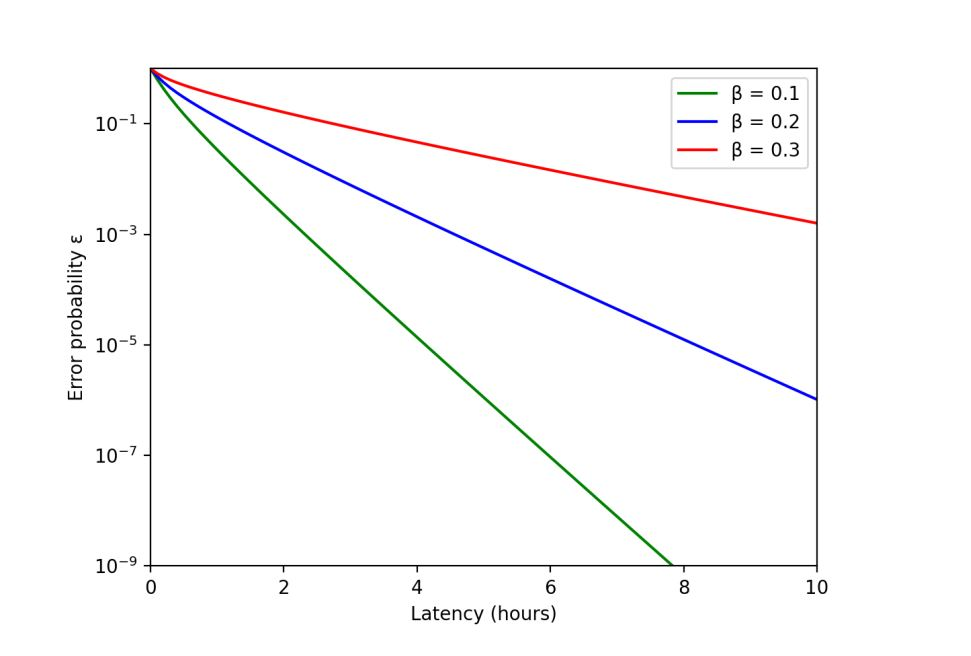
\includegraphics[width=0.8\linewidth]{Fig/09/F1}
        \caption{Bitcoin’s latency–security trade-off for different $\beta$ assuming $\delta = 0$. We set $\lambda$ to be $6$ blocks per hour, as in Bitcoin.}
        \label{fig:f1}
    \end{figure}
\end{center}
In the general case when $\delta > 0$, the private attack is no longer the worst-case attack in terms of success probability. However, it still provides a lower bound on the error probability, which consequently sets a lower bound on the latency for a given error probability. Both the error probability and latency tend to increase as $\delta$ increases due to increased forking caused by propagation delays in the network.\\
From a practical perspective, what is more interesting are the upper bounds on the error probability and latency, as they provide practical guidance for users of Bitcoin to determine when a transaction can be considered confirmed with a desired level of confidence. \href{https://arxiv.org/pdf/2011.14051.pdf}{Recent research} has derived such upper bounds, which are fairly close to the lower bounds implied by the private attack.\\
For example, consider a scenario where the adversary controls $10\%$ of the total mining power and the block propagation delays are within $\delta = 10$ seconds. With these settings, a Bitcoin block can be confirmed with less than $10^{-3}$ error probability after approximately $5$ hours and $20$ minutes. For an even higher level of confidence, a block can be confirmed with less than $10^{-10}$ error probability after approximately $12$ hours and $15$ minutes.\\
Figure \ref{fig:f2} illustrates the security-latency trade-off as implied by both the lower and upper bounds. The plot shows how the error probability decreases with increasing latency and how the upper and lower bounds are relatively close, providing a reasonable estimate of the confirmation time for a desired level of security.
\begin{center}
    \begin{figure}
        \centering
        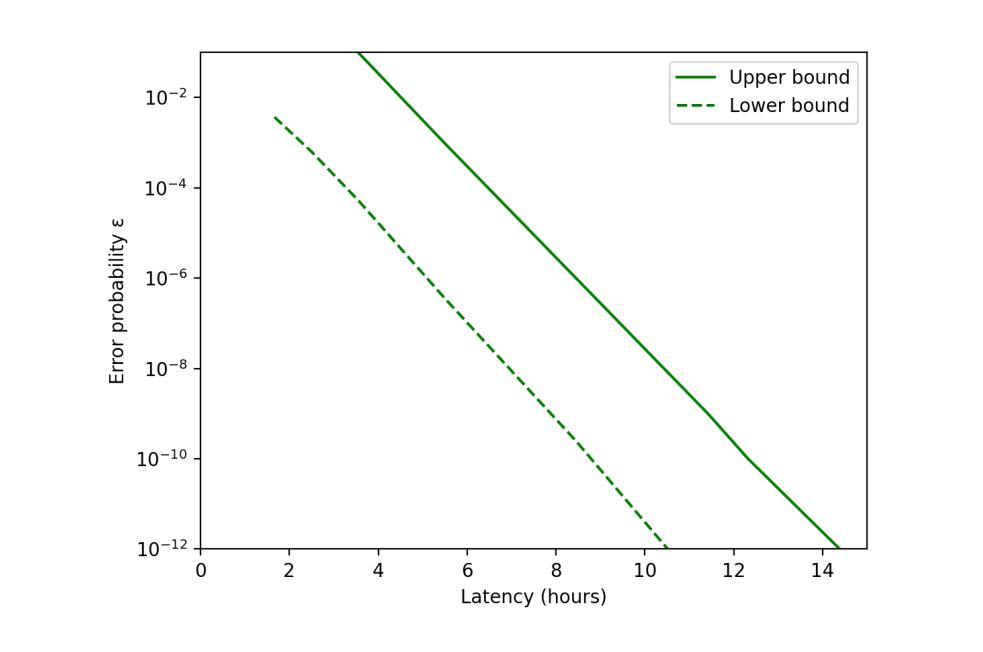
\includegraphics[width=0.8\linewidth]{Fig/09/F2}
        \caption{Bitcoin’s latency–security trade-off for $\beta = 0.1$ when $\delta > 0$. We set $\lambda$ to be $6$ blocks per hour as in Bitcoin and $\delta = 10$ seconds. The lower bound on latency is derived from the private attack, while the upper bound is borrowed from \href{https://arxiv.org/pdf/2011.14051.pdf}{this work}.}
        \label{fig:f2}
    \end{figure}
\end{center}
\section{Prism: Fast Confirmation}
Lecture 8 introduces Prism 1.0, a blockchain protocol with two types of blocks: transaction blocks and proposer blocks. These blocks separate the security and payload aspects of the longest chain protocol. The proposer blocks serve two roles: they act as leaders for the "round" and provide confidence to ancestor blocks through the k-deep confirmation rule. Additionally, they vote for all ancestor blocks via parent link relationships. The full Prism protocol further decouples voting from proposer blocks by introducing separate voter blocks. The proposer block tree anchors the blockchain, and each proposer block contains reference links to transaction blocks and a reference to its parent proposer block. Honest nodes mine proposer blocks following the longest chain rule in the proposer tree. The level of a proposer block represents its distance from the genesis proposer block, while the height of the proposer tree is the maximum level containing any proposer blocks. To determine the ordering of proposer blocks and transactions, one leader proposer block is elected from each level, forming the leader sequence up to the height of the proposer tree, determined by the voter chains.
\begin{center}
    \begin{figure}
        \centering
        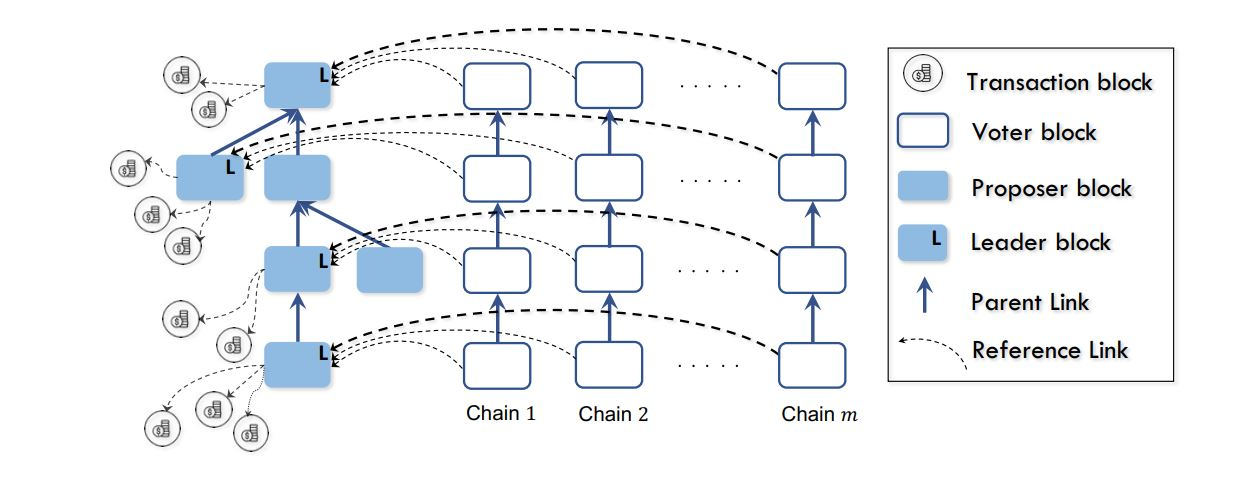
\includegraphics[width=0.8\linewidth]{Fig/09/F3}
        \caption{Factorizing the blocks into three types of blocks: proposer blocks, transaction blocks, and voter blocks.}
        \label{fig:f3}
    \end{figure}
\end{center}
\begin{itemize}
    \item Prism 1.0 introduces two types of blocks: transaction blocks and proposer blocks.
    \item These blocks decouple the security and payload aspects of the longest chain protocol.
    \item Proposer blocks have two roles: proposing as leaders for the round and adding confidence to ancestor blocks through the k-deep confirmation rule.
    \item Proposer blocks also vote for all ancestor blocks through parent link relationships.
    \item The full Prism protocol further separates voting from proposer blocks by introducing separate voter blocks.
    \item The proposer block tree anchors the blockchain and contains reference links to transaction blocks and a parent proposer block reference.
    \item Honest nodes follow the longest chain rule to mine proposer blocks in the proposer tree.
    \item The level of a proposer block represents its distance from the genesis proposer block, and the height of the proposer tree is the maximum level with proposer blocks.
    \item One leader proposer block is elected from each level to determine the ordering of proposer blocks and transactions.
    \item The leader sequence, determined by voter chains, comprises leader proposer blocks up to the height of the proposer tree, independent of the chain structure of proposer blocks to avoid deadlocks.
\end{itemize}
In Prism, there are $m$ voter chains, where $m >> 1$ is a fixed parameter set by the system designer. The value of $m$ determines the level of parallelism in the voting process, and a larger $m$ leads to shorter confirmation latencies. The choice of $m$ is typically limited by network bandwidth and memory management considerations. For example, a full-stack implementation of Prism may use $m = 1000$.\\
New voter blocks are continuously mined on each voter chain, following the longest chain rule. Each voter block serves as a vote for a proposer block by containing a reference link to that proposer block. The voting process has specific requirements: 
\begin{enumerate}
    \item A vote is valid only if the voter block is part of the longest chain in its respective voter tree.
    \item Each voter chain votes for exactly one proposer block at each level.
    \item Each voter block votes for all proposer levels that have not been voted by its parent.
\end{enumerate}
The leader block at each level is determined by the proposer block that receives the highest number of votes among all proposer blocks at that level. In the case of ties, the leader is chosen based on the hash of the proposer blocks. The elected leader blocks establish a unique ordering of the transaction blocks, forming the final ledger of the Prism blockchain.\\
In Prism, cryptographic sortition is employed to prevent the adversary from concentrating its mining power on specific types of blocks or voter chains. To form a "superblock," a miner combines three components: a transaction block, a proposer block, and a voter block from the $i$-th voter tree, where $1 \leq i \leq m$. A superblock is considered successfully mined if its hash value, computed using a nonce, is less than the threshold value $T_{tx} + T_{prob} + mT_{v}$.\\
Once a superblock is successfully mined, it is identified as one of the following based on its hash output. (See Figure \ref{fig:f4} for an illustration):\\
\begin{itemize}
    \item A proposer block if the hash output is less than $T_{prop}$.
    \item A transaction block if the hash output falls within the range $[T_{prob}, T_{tx} + T_{prob})$.
    \item A voter block on the $i$-th voter tree if the hash output falls within the range $[T_{tx} + T_{prob} + (i − 1)T_{v}, T_{tx} + T_{prob} + iT_{v})$, where $1 \leq i \leq m$.
\end{itemize}
As we said above, Prism is a blockchain protocol that decouples the security and payload aspects of the longest chain protocol. It introduces two types of blocks: transaction blocks and proposer blocks, which act as leaders and voters in the security aspect. Additionally, there are m voter chains to parallelize the voting process, and cryptographic sortition prevents the adversary from concentrating mining power on specific blocks or voter chains. The protocol ensures a unique ordering of transaction blocks and enables ledger sanitization after the ledger has stabilized.\\
\\
More details are listed below:
\\
\begin{enumerate}
    \item Prism employs cryptographic sortition to prevent the adversary from focusing its mining power on specific blocks or voter chains.
    \item Superblocks are formed by combining a transaction block, a proposer block, and a voter block from the $i$-th voter tree ($1\leq i \leq m$).
    \item The successful mining of a superblock is determined by the hash output being less than specific threshold values $T_{prob}$, $T_{tx}$, and $T_{v}$.
    \item The probability of a superblock being identified as a proposer block, a transaction block, or a voter block on the $i$-th voter tree is proportional to $T_{prob}$, $T_{tx}$, and $T_{v}$, respectively.
    \item The transaction target difficulty ($T_{tx}$) is set easy, allowing for parallel mining of transaction blocks, while the proposer and voter chain target difficulties ($T_{prop}$ and $T_{v}$) are set high for security.
    \item The Prism protocol decouples the process of mining blocks from validating transactions, as the miner cannot validate a block before mining due to the non-chain structure of proposer blocks.
    \item After a confirmed leader sequence of proposer blocks is established, the ordering of transaction blocks becomes uniquely determined, enabling ledger sanitization and validating individual transactions.
\end{enumerate}
Overall, Prism combines parallelism, security, and decoupling to achieve efficient and secure transaction processing in a blockchain protocol.
\begin{center}
    \begin{figure}
        \centering
        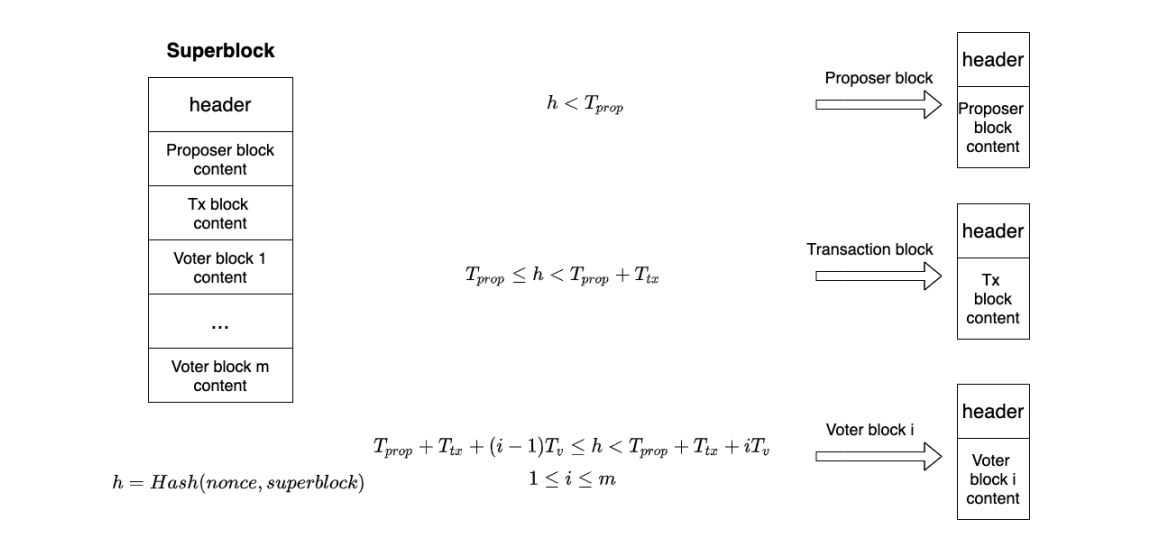
\includegraphics[width=0.8\linewidth]{Fig/09/F4}
        \caption{Superblock containing a transaction block, a proposer block and m voter blocks is “$(m+2)$-for-one” mined; the resulting cryptographic sortition identifies the type of the block as the winner of the mining process.}
        \label{fig:f4}
    \end{figure}
\end{center}
\section{Fast confirmation rule in Prism}
In summary, Prism's parallel voting scheme allows for faster confirmation latency. By leveraging the law of large numbers, votes can be considered even if they are not fully stabilized, providing security while minimizing latency. However, these techniques need to be carefully analyzed to ensure the protocol's robustness against attacks. More details are listed below:
\begin{enumerate}
    \item \textbf{Parallel Voting Scheme in Prism:} The parallel chain structure of the voting scheme in Prism allows for low confirmation latency. Votes accrue in parallel, unlike Bitcoin's sequential voting approach, leading to faster confirmation times for a fixed level of security.
    \item \textbf{Simple Case of Confirmation Latency:} Let's consider a simple case in Prism where a single honest proposer block ($B_{p}$) at level one is mined at time $0$. In Prism, $B_{p}$ can be confirmed if no other proposer block at level one receives more votes than it. However, this naive solution is not operational since the confirmation depends on the future.
    \item \textbf{Principled Confirmation Rule:} A principled confirmation rule that balances security and fast latency is needed. Waiting until each vote stabilizes by being k-deep in their chains (similar to Bitcoin) results in high latency. However, it's not necessary to wait for each vote to stabilize fully.
    \item \textbf{Leveraging the Law of Large Numbers:} Even if each vote is ephemeral (with a small value of $k$, e.g., $k = 2$ or $3$), the averaging of all votes ensures overall security. This phenomenon is analogous to the law of large numbers or boosting in machine learning, where combining many low-precision classifiers creates a high-precision classifier.
    \item \textbf{Analysis of a Simple Attack:} Consider a scenario where an honest proposer block $H$ refers to a transaction block $TB$ and is currently isolated at its level, meaning no other public proposer block exists at the same level. Block $H$ starts collecting votes, each from the longest chain of its respective voter tree (See Figure \ref{fig:f5}(a)). The adversary attempts a private attack by mining a private proposer block $A$ at the same level and forking off private alternate chains on each voter tree. It then sends its vote to block $A$. The adversary continues to mine on each voter alternate chain to overtake the public longest chain and shift the vote from $H$ to $A$. The attack is successful if the adversary gets more votes on $A$ than on $H$.
\end{enumerate}
\begin{center}
    \begin{figure}
        \centering
        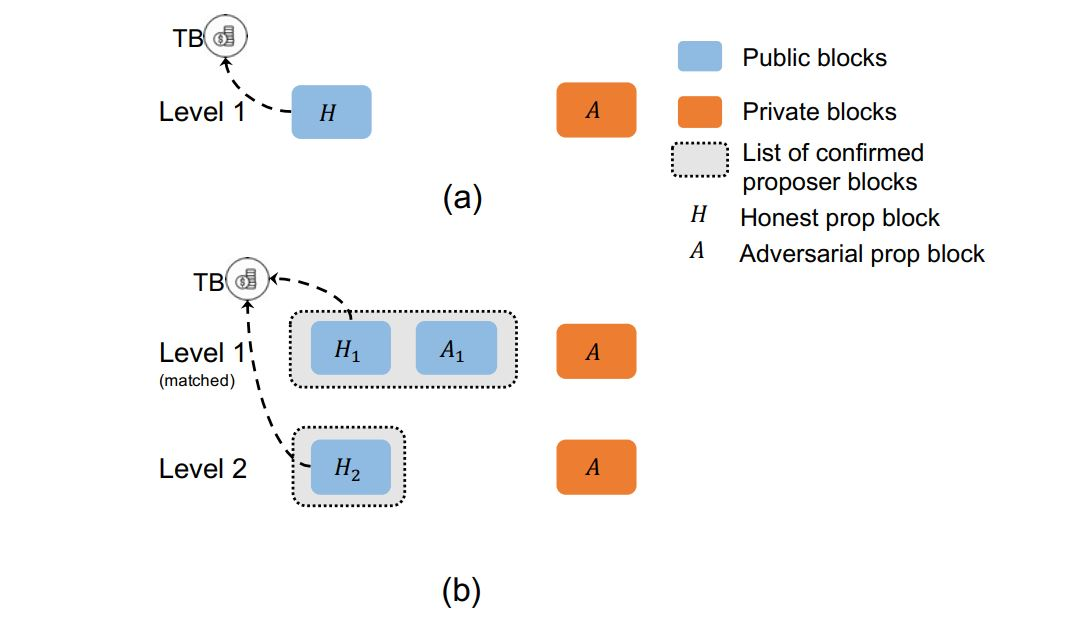
\includegraphics[width=0.8\linewidth]{Fig/09/F5}
        \caption{(a) Transaction block is referred to by an isolated honest proposer block. (b) Transaction block is referred to as a non-isolated proposer block but on the next level, there is an isolated proposer block. Note that since $H_{2}$ is honest, it refers to all unconfirmed transaction blocks, i.e., $TB$.}
        \label{fig:f5}
    \end{figure}
\end{center}
\subsection{Fast confirmation rule}
The use of multiple voter chains in Prism reduces confirmation latency while maintaining security. By leveraging Nakamoto's calculations and employing averaging principles, the protocol achieves faster confirmation times without compromising robustness against attacks. In summary, we can say:
\begin{enumerate}
    \item \textbf{Attack Analogy to Nakamoto's Private Attack:} The attack in Prism, with m chains, can be seen as the multi-chain analog of Nakamoto's private attack on Bitcoin. Instead of a single race between the honest chain and the private chain, we have m races in Prism.
    \item \textbf{Using Nakamoto's Calculations for Determining Waiting Depth:} Nakamoto's calculations on the success probability of an attack on a single chain can help determine how deep we should wait for votes to confirm the proposer block H in Prism. For tolerable adversary power ($\beta = 0.3$), the reversal probability in a single chain is $0.45$ when a block is $2$-deep.
    \item \textbf{Latency Reduction with Multiple Voter Chains:} With $m = 1000$ voter chains and each vote being $2$-deep, the expected number of chains that can be reversed by the adversary is $450$. The probability that the adversary can reverse more than half the votes ($500$) is about $10^{-3}$. Thus, to achieve $\epsilon = 10^{-3}$, we only need to wait for $1000$ votes each $2$-deep, resulting in much shorter latency than waiting for $24$ block depths for each vote to be reversed with a probability of $10^{-3}$.
    \item \textbf{Conceptual Similarity to Averaging Classifiers:} The reduction in latency in Prism is conceptually similar to averaging many unreliable classifiers to form a strong aggregate classifier. With more voter chains, individual votes need less certainty of permanence, leading to reduced confirmation time without sacrificing security.
    \item \textbf{Ensuring Security:} Despite the reduced waiting depth for votes, each voter chain in Prism is still operating slowly enough to tolerate adversarial hash power ($\beta$). This ensures security against attacks even with shorter confirmation times.
\end{enumerate}
\subsection{Tentative Confirmation rule}
By employing the tentative confirmation rule based on the function h(t), Prism achieves a confirmation time that is observable and accurate even in the absence of direct time information in the blockchain. This allows for efficient and secure confirmation of proposer blocks in the protocol.\\
\begin{enumerate}
    \item \textbf{Tentative Confirmation Rule:}  To confirm proposer block $B_{p}$ at time $t^{\ast}$, we look for a time $t^{\ast}$ where the function $h(t) = \frac{1}{2}$. The function $h(t)$ calculates the fraction of stabilized votes (or effective votes from one voter chain) at time $t$.
    \item \textbf{Closed Form Expression for $h(t)$:} The closed-form expression for $h(t)$ can be derived in the appendix and depends only on the mining rate $\lambda$ and the tolerable adversary hash power fraction $\beta$.
    \item \textbf{Numerical Calculation:} For instance, when $\beta = 0.3$, we can numerically calculate $t^{\ast} \approx \frac{3}{\lambda}$, resulting in a confirmation time that is a small factor of the average inter-block arrival time.
    \item \textbf{Time Estimation:} Time is not directly observable in a proof-of-work blockchain due to potential inaccuracies or adversarial manipulation of timestamps in blocks. However, it can be estimated from the growth of the voter chains in Prism.
    \item \textbf{Accurate Estimation:} The large number of voter chains in Prism ensures accurate estimation of time even for short periods due to the law of large numbers. The total mining rate of all voter chains is $m\lambda$, and on average $m\lambda$ voter blocks are mined within $t$ units of time.
    \item \textbf{Block-Based Confirmation Rule:} Using the conversion from time to blocks, a block-based confirmation rule becomes observable and practical.
\end{enumerate}
\subsection{Final confirmation rule}
Exactly, in Prism, the tentative confirmation rule states that proposer block $B_{p}$ will be confirmed when $mt^{\ast}\lambda$ voter blocks are mined and there is no competing proposer block at the same level. As mentioned earlier, $t^{\ast}$ is a function of the mining rate $\lambda$ and the tolerated adversary hash power fraction $\beta$. For example, when $\beta = 0.3$, it is numerically calculated that $t^{\ast} \approx \frac{3}{\lambda}$.\\
Therefore, under these conditions, Prism confirms the proposer block $B_{p}$ once $3m$ voter blocks are mined, ensuring a secure and efficient confirmation process. The large number of voter chains ($m$) and the ability to estimate time accurately through voter chain growth contribute to the reduction in confirmation latency while maintaining security against adversarial attacks.
\section{Non-isolated Proposer Block}
Consider now the case when the transaction block $TB$ is referred to by an honest proposer block $H_{1}$  which is not isolated at its level, i.e. $H_{1}$ is matched by an adversarial public proposer block $A_{1}$ (the competing proposer block could also be honest). This matching could persist for $L$ levels until reaching a level when there is an isolated honest proposer block. See Figure \ref{fig:f5}(b) for the special case of $L = 1$. Let us separately consider the life cycle of an honest transaction vs. a double-spent one.
\subsection{Honest transaction}
For confirmation of an honest transaction, a naive approach would be to wait until we can definitively confirm either $H_{1}$ or $A_{1}$. However, this approach may be slow due to adversarial attacks attempting to balance votes between $H_{1}$ and $A_{1}$. A key insight is that for honest transactions, we don't need to know which of $H_{1}$ and $A_{1}$ will be confirmed—only that one of them will be confirmed. This weaker form of list confirmation works because if $A_{1}$ eventually gets confirmed, a later honest proposer block can still refer to $TB$.\\
To confirm an honest transaction at level $i$, we need two events:
\begin{enumerate}
    \item \textbf{List confirmation of all levels up to $i$:} Once we have list-confirmed a set of proposer blocks at level $i$ referring to $TB$ (e.g., either $H_{1}$ or $A_{1}$ will be the leader), we know that no other block can be the leader at that level. However, list confirmation alone is not enough if the transaction is not present in all ledgers. In that case, we also need to wait for an isolated honest proposer level where the proposer block will include $TB$ in the ledger.
    \item \textbf{Isolated honest proposer level:} Once this isolated honest proposer level is confirmed, and all the preceding levels are list-confirmed, we can be sure that $TB$ will appear in the final ledger.
\end{enumerate}
The confirmation latency is thus the maximum of two parts:\\
\begin{enumerate}
    \item \textbf{List confirmation:} We quickly confirm that the adversary cannot produce a private block $A$ with more votes than the votes of public blocks $H_{1}$ and $A_{1}$. The logic is similar to the case of an isolated honest proposer block discussed above, viewing the situation as a race between honest nodes voting for the public blocks $H_{1}$ or $A_{1}$ and the adversary voting for $A$. Adversarial actions (e.g., presenting $H_{1}$ to half the honest nodes and $A_{1}$ to the other half) can cause the number of votes to be evenly split between $H_{1}$ and $A_{1}$, which can slow down list confirmation, albeit not significantly.
    \item \textbf{Isolated honest proposer level:} For example, in Figure \ref{fig:f5}(b), if we wait until level $2$, we see an isolated public proposer block $H_{2}$, which can be fast confirmed. At this point, we know that the final leader sequence at levels $1$ and $2$ is either $H_{1}$, $H_{2}$ or $A_{1}$, $H_{2}$, both of which contain our honest transaction since $H_{2}$ refers to all previous unconfirmed transaction blocks.
\end{enumerate}
\subsection{Double-spent transaction}
For confirmation of double-spent transactions, we require stronger conditions than those mentioned earlier. Instead of list confirmation, we need unique block confirmation, which confirms which block at a proposer level will be the ultimate leader. This is achieved once list confirmation occurs, and one of the list-confirmed blocks can be reliably declared the winner. If one of the public proposer blocks $H_{1}$ or $A_{1}$ gathers many more votes than the other block, then we can quickly confirm a unique leader, even for double-spent transactions.\\
However, certain adversarial attacks, like balancing the votes on $H_{1}$ and $A_{1}$, can cause the number of votes to be evenly split between $H_{1}$ and $A_{1}$. In such cases, we cannot fast confirm a leader block. In this scenario, we must wait until every vote on $H_{1}$ and A1 stabilizes, at which point either $H_{1}$ or $A_{1}$ is confirmed, and only one of the double-spent transactions is accepted. A content-dependent tie-breaking rule can be used to break ties after votes are stabilized, ensuring that the final decision on the accepted transaction is deterministic.
\section{Scaling latency via Prism}
The latency of Prism, denoted as $\tau_{Prism}$, under the "normal path" (i.e., when there is a single proposer block for a level) is given by:\\
\begin{equation*}
    \tau_{Prism} = O(\frac{1}{\lambda}),
\end{equation*}
where $\lambda$ is the mining rate. This latency is independent of the error probability $\epsilon$ when the parameter m (number of voter chains) is chosen to be sufficiently large. The constant hidden in the $O(·)$ notation depends only on the fraction of tolerable adversary hash power $\beta$.\\
Compared to Bitcoin, Prism achieves faster confirmation because it only needs to wait until the effective vote $h(t)$ is greater than $0.5$. The use of many voter chains in Prism allows the application of the law of large numbers horizontally (in space). This means that the majority of the voter chains have voted for a proposer block irreversibly, and hence we can confirm the block with high probability.\\
In contrast, in Bitcoin, there is only one chain, so we have to wait until $h(t)$ is $1 - \epsilon$ to guarantee a small deconfirmation probability $\epsilon$. In Bitcoin, the law of large numbers is applied vertically (in time), as discussed in Lecture 6.\\
The comparison between Bitcoin and Prism latency is illustrated in Figure \ref{fig:f6}. In summary, by using many voter chains, Prism eliminates the $\ln(\frac{1}{\lambda})$ term present in Bitcoin's latency. This decouples latency from security and achieves fast confirmation.
\begin{center}
    \begin{figure}
        \centering
        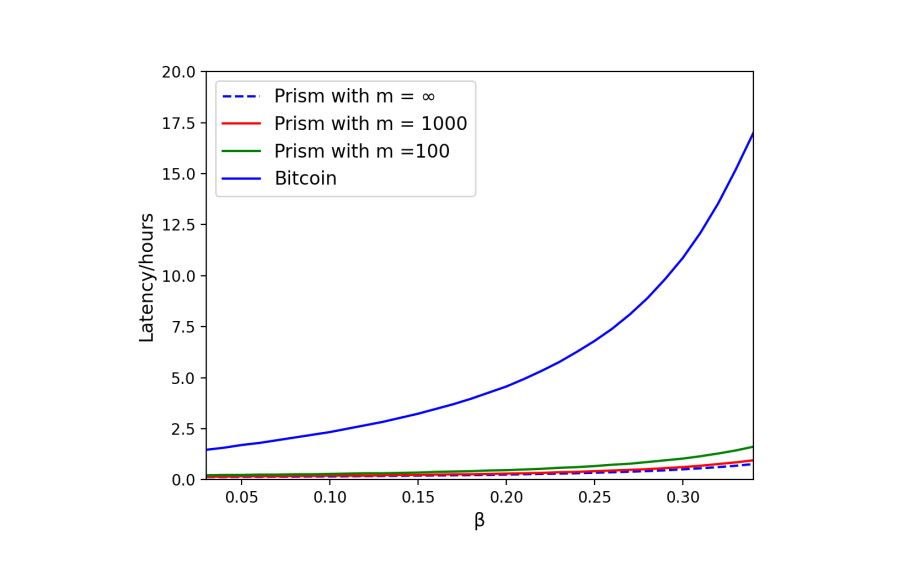
\includegraphics[width=0.8\linewidth]{Fig/09/F6}
        \caption{Comparison between Bitcoin and Prism latency under various values of $\beta$. We set $\lambda$ to be 6 blocks per hour and the error probability $\epsilon = 10^{−3}$. This also justifies the choice of $m$ in the \href{https://arxiv.org/abs/1909.11261}{implementation of Prism}.}
        \label{fig:f6}
    \end{figure}
\end{center}